\documentclass[12pt,a4paper]{report}
\usepackage[left=1in,right=1in,top=1in,bottom=1in]{geometry}
\usepackage{xr}
\usepackage{graphicx}
\usepackage[table,xcdraw]{xcolor}
\usepackage{microtype}
\usepackage{float}
\usepackage{url}
\usepackage{import}
\usepackage{gensymb}
\usepackage{graphicx}
\usepackage{caption}
\usepackage{pdfpages}
\usepackage{listings}
\usepackage{amsmath}
\usepackage{rotating}
\usepackage{pdfpages}
\usepackage{subcaption}
\usepackage{parskip}
\usepackage{booktabs}
\usepackage{tabularx}
\usepackage[toc,nonumberlist]{glossaries}

\parskip=1.1\baselineskip
\setcounter{secnumdepth}{3}

\begin{document}	
	\bibliographystyle{plain}
	\lstset{
		frame=single, 
		breaklines=true, 
		numbers=left}
	\captionsetup{labelfont=bf}

	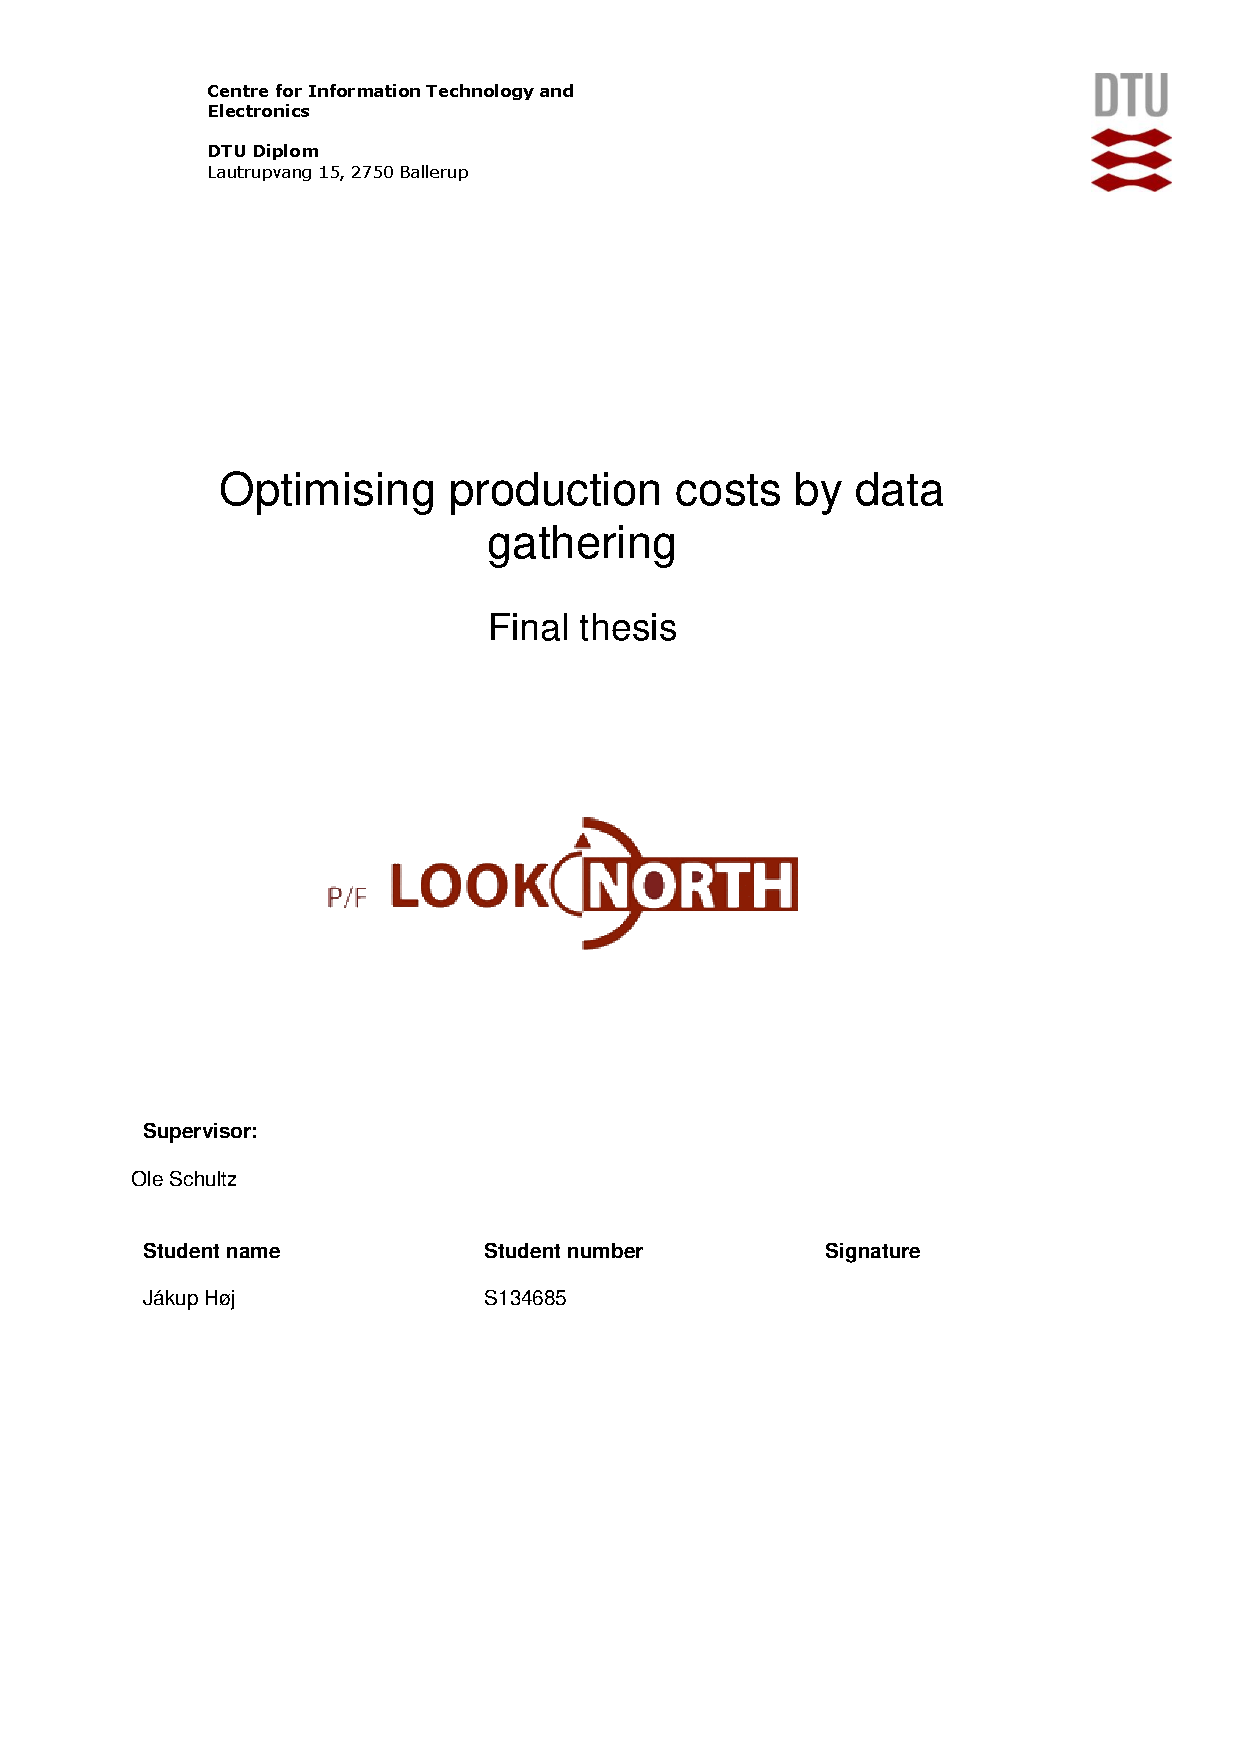
\includepdf[pages=-,]{pdfs/cover.pdf}
	
	\begin{abstract}
		This report, and the code included on the CD attached to it, is the final product produced for the final project as an IT engineer at the Technical University of Denmark, Ballerup Campus.
		
		The purpose of the project is to demonstrate my ability to analyse, design and implement a solution to the problem case delivered to me by P/F Looknorth.
		
		The problem to be solved is to make a solution so that the production machines operate at the same good level, but stabilising the oil consumption. 	
\end{abstract}
	
	\tableofcontents
		
	\chapter{Introduction} \label{chap:intro}
\section{About Looknorth}
Looknorth is a company located in the Faroe Islands, and was founded in 2000. The company's factory is located in Klaksvík, where all their production is done. Looknorth's production is mainly polysterne products, where the majority of the products are made for the salmon industry, which is growing at a rapid rate in the Faroe Islands.
Looknorth is a company that is expanding gradually. Their storage was expanded in 2011.
Looknorth's production is running 24/7,

How the machines work

How how much oil is used, and show why the more energy used is possible and expensive.

\section{Project Start}
In this project, a system is built that can:
\begin{enumerate}
	\item Show how much oil is used for the current production.
	
	\item Give the machines operator an indication of the current oil consumption. Showing wheter the consumption is too high or low for the given combination of products that are currently in production.
	
	\item Take into account that the production will scale over time.
	
	\item Allow the users to increase the production capacity and catalouge easily.
\end{enumerate}

To build such an application, a distributed systems approach has to be used.

The whole system will consist of: 

\begin{description}
	\item[The sensor programs:] These sensor programs will detect changes in two environments. The machines and the oil consumption.
	\item[The server programs:] The server programs will handle persistance, and business logic, such as calculate the recommended oil consumption.
	\item[The user programs:] A program for the machine operator to see the oil consumption. 
	A program for the administrator, to add new products and increase production capacity, as well as the possibility to make manual changes to the oil consumption recommendations. 
\end{description} 

\section{Planning} 
		 		     			 		    \include{chapters/problemformulation}
	\include{chapters/problemanalysis}
	\include{chapters/delimitation}
	\include{chapters/problemsolution}								    \include{chapters/acceptancetesting}
				
	\include{chapters/conclusion}						
	\glsaddall
	\printglossaries
	
	\bibliography{refs/references}

	\appendix
	
	//appendix here
	\nocite{*}
\end{document}